\sectionlang{sv}{Instuderingsfrågor}
\sectionlang{en}{Preparatory study assignments}
\label{sec:instudering}
\lang{sv}{
Det är viktigt att ni innan laborationen har en idé om vad ni vill ta
reda på och hur ni vill gå till väga. Därför skall ni senast en studievecka
före ert laborationstillfälle ha besvarat nedanstående frågeställningar
skriftligen.
Variablerna $x_1$, $x_2$ och $x_3$
%$\aleph$, $\beth$ och $\daleth$
är era individuella födelseår
(2-siffrigt), födelsemånad och födelsedag respektive. Ange
laborationsdatum i inlämningen.

\begin{enumerate}
\item Vad händer ifall ni försöker följa reaktionen vid för hög
  temperatur?
\item Vad händer ifall ni försöker följa reaktionen vid för hög
  jonstyrka?
\item Om ni uppmäter en hastighetskonstant för Reaktion \ref{eq:equilibrium} vid
  jonstyrkan $I = \SI{0.05}{\mole\per\kg}$, hur skall ni då ändra
  jonstyrkan så att den observerade hastighetskonstanten minskar med 30\%?
\item Vad är jämviktskoncentrationen \ce{FeSCN^{2+}} ifall
  $[\ce{SCN^{-}}]_{tot} = 10 x_1~\si{\micro\Molar}$ och 
  $[\ce{Fe^{3+}}]_{tot} = \SI{1.5}{\milli\Molar}$, vilken absorbans ger det?
% \item Vad är
%   $\frac{\gamma_\ce{FeSCN^{2+}}}{\gamma_\ce{Fe^{3+}}\gamma_\ce{SCN^-}}$
%   för $I = x_1~\si{\milli\mole\per\kg}$?
\item Vad är $\frac{[\ce{Fe^{3+}}]}{[\ce{FeOH^{2+}}]}$ vid pH $x_2$?
\item Vad är $[\ce{Fe_2(OH)_2^{4+}}]$ vid pH 2 ifall
  $[\ce{Fe^{3+}}]_{tot} = x_3~\si{\milli\Molar}$?\footnote{
Alternativ 1: försumma bildandet av \ce{FeOH^{2+}}. Alternativ 2: ställ upp ekvationer
för jämvikterna och utnyttja bevarandet av järnatomerna, lös
exempelvis med WolframAlpha.
}
% \item Vad sker med jonstyrkan under reaktionsförloppet i en vattenlösning
%   med stökiometriska mängder järn(III)perklorat och natriumtiocyanat med
%   mycket små halter av åskådarjoner? Hur påverkar det
%   hastighetskonstanten $\SYMkf$?
\item Vad är tänkbara initialkoncentrationer (dvs. vad tror ni kommer att
  fungera bra)? Dessa kan sedan justeras baserat på erhållna data. Se
  \cref{fig:fe} för val av pH.
\item Vad är jonstyrkan vid $t=0$? Förväntar ni er att den kommer att
  förändras mycket under reaktionsförloppet?
\item Vad är absorbansen vid $t=\infty$ för era föreslagna
  koncentrationer? Vid vilken transmittans tror ni att ni har bäst
  känslighet i er detektor? Vilken absorbans motsvarar det? (Om
  absorbansen är olämplig: ändra då era föreslagna intialkoncentrationer)
\end{enumerate}

Beskriv era resonemang utförligt och motivera eventuella approximationer
(t.ex. om ni antar en koncentration konstant pga stort överskott).
}
\lang{en}{
It is important that you have an idea of what you want to take before the lab
Find out and how you want to go. That's why you will receive a student voucher at the latest
Prior to your laboratory session, have answered the questions below
In writing.
The variables $x_1$, $x_2$ and $x_3$ are your individual birth years
(2-digit), birth month and birthday respectively. Enter
Laboratory date in submission.

\begin{enumerate}
\item What happens if you try to follow the reaction too high
  temperature?
\item What happens if you try to follow the reaction too high
  Ion strength?
\item If you measure a rate constant for Reaction \ref{eq:equilibrium} at
  Ion strength $ I = \SI{0.05}{\mole\per\kg}$, how should you change
  Ionic strength so that the observed rate constant decreases by 30\%?
\item What is the equilibrium concentration \ce{FeSCN^{2+}} if
  $[\ce{SCN^{-}}]_{tot} = 10 x_1 ~ \si{\micro\Molar} $ and
  $[\ce{Fe^{3+}}]_{tot} = \SI{1.5}{\milli\Molar} $, which absorbance gives it?
% \item What is
% $ \ Frac {\ n {c} {FeSCN ^ {2 +}}} {\ gamma_ \ ce {Fe ^ {3 +}} \ gamma_ \ ce {SCN ^ -}} $
% For $ I = x_1 ~ \ say {\ milli \ mole \ per \ kg} $?
\item What is $ \frac{[\ce{Fe^{3+}}]}{[\ce{FeOH^{2+}}]} $ at pH $x_2$?
\item What is $[\ce{Fe_2(OH)_2^{4+}}]$ at pH 2 if
  $[\ce{Fe^{3+}}]_{tot} = x_3 ~ \si{\milli\Molar}$?\footnote{
Option 1: neglect the formation of \ce{FeOH^{2+}}. Option 2: set up equations
For the equilibrium and utilizing the conservation of the iron atoms, solve
For example with WolframAlpha.
}
% \item What happens to the ionic strength during the course of the reaction in an aqueous solution
% With stoichiometric amounts of iron (III) perchlorate and sodium thiocyanate with
% Very small levels of sightings? How does it affect
% Rate constant $ \SYMkf $?
\item What are possible initial concentrations (ie what do you think will be
  works fine)? These can then be adjusted based on data obtained. See
  \cref{fig:fe} for selection of pH.
\item What is the ionic strength at $t=0$? Do you expect it to be
  Change a lot during the course of the reaction?
\item What is the absorbance at $t = \infty$ for your proposed
  Concentrations? At what transmittance do you think you are the best?
  Sensitivity in your detector? What absorbance does it correspond to? (If
  Absorbance is inappropriate: change your suggested initial concentrations)
\end{enumerate}

Describe your reasoning in detail and motivate possible approximations
(For example, if you assume constant concentration due to large excess).
}
\begin{figure}
  \centering
  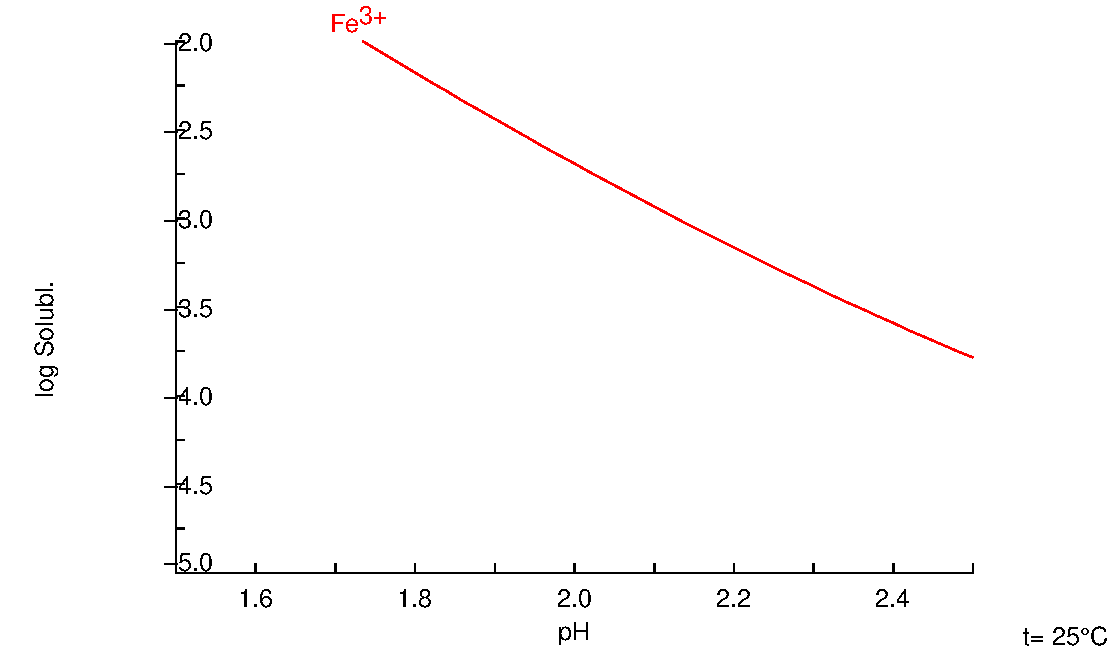
\includegraphics[scale=0.4]{fig/fe.pdf}
  \caption{Löslighetsdiagram för järn(III)}
  \label{fig:fe}
\end{figure}

%%% Local Variables:
%%% mode: latex
%%% TeX-master: "../main"
%%% ispell-local-dictionary: "swedish"
%%% End:
